
\subsection{Autoencoder}

Autoencoders are neural networks used to learn efficient representations of data.
Through unsupervised learning, autoencoders do not need labeled data to function.
Autoencoders accomplish this by lowering the dimensional complexity of the data, enabling it to store data representations more efficiently.
Due to this ability, autoencoders are well suited for dimensional reduction of data.
Autoencoders learn to represent data in a \textit{coding}.
This \textit{coding} has a much lower dimensionality than the original data
\cite[p.~506-508]{Geron2017}.

Autoencoders are composed of 2 parts; the encoder and the decoder.
The encoder maps the input data representation to the \textit{coding}, while the decoder maps the coding values back through data reconstruction.
The encoder takes the input data and reduces the feature mapping to store the reduced data representation in the coding layer.
The data is then sent from the coding layer to the decoder, where the decoder attempts to reverse the mapped data back to the original input data.
By doing this, the encoder efficiently maps essential data features in the coding layer, using far lower dimensionality than the original data.
The decoder then efficiently reconstructs the input data using only the dimensionally reduced data in the coding layer
\cite[p.~506-508]{Geron2017}.


\begin{figure}[h!]
    \centering
    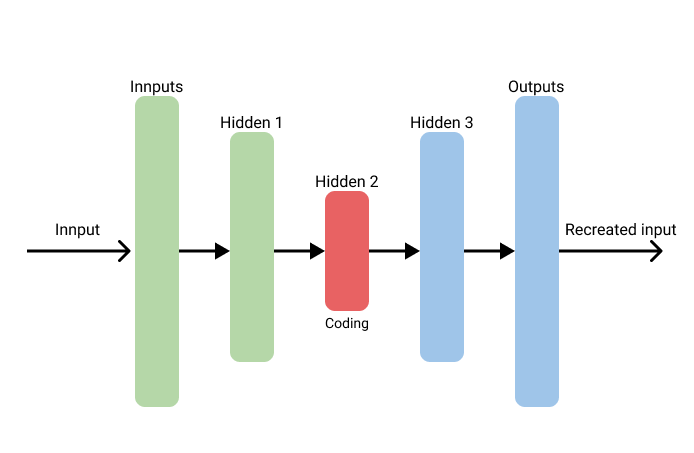
\includegraphics[width=0.7\textwidth]{./sections/BT/figures/Autoencoder.png}
    \hfill
    \caption{Figure of a Stacked Autoencoder architecture with one hidden encoder layer, and one hidden decoder layer.}
    \label{fig:stacked_autoencoder_arch}
\end{figure}

Through feature mapping, the encoder becomes an efficient feature detector and extractor.
Due to the reduced dimensionality of the coding, the encoder becomes sufficient at reducing the noise within the data, extracting the most important features.
As a future extractor, autoencoders are well suited for pre-training neural networks, extracting essential features.
At the same time, autoencoders can become successful generative models.
The decoder is proficient at reconstructing input data from the coding layer representation, meaning it can also generate new data.
The reconstructive abilities of the decoder enable the generative model to create new data, similar to the training data used when creating the model
\cite[p.~506-508]{Geron2017}.
